%%% -*-LaTeX-*-

\chapter{Sequence Construction}

With an exact count of viable sequences for tier one, two, and three designs, a mapping from natural numbers to valid trial sequences is now a possibility. Such a mapping would prove valuable for guaranteeing a uniform distribution of samples, as well as generating solutions more efficiently. This chapter presents an algorithm that is guaranteed to generate uniformly-distributed solutions to tier one, two, and three designs. This is accomplished by randomly sampling natural numbers from the uniform distribution in the range of $[0, s)$, then generating the unique trial sequence associated with that number. Lastly, the generated trial sequence is checked against design constraints (if any exist), to ensure that no violations exist in the generated sequence.


\section{Enumerating Permutations and Combinations}

There are several steps involved in constructing a solution based on a natural number. In this section, we will review methods for generating the $n^{th}$ permutation or combination of a set, as well as mapping individual natural numbers to a unique set of numbers that covers the same space using modular arithmetic. These techniques form the basic building blocks for the final construction algorithm.

\subsection{Interval Mapping}

The construction algorithm will repeatedly need to take a single number and map it into a unique combination of multiple numbers, each from a possibly different range. We will refer to this process as \textit{interval mapping}.

Suppose we have $n$ numeric intervals, each ranging from $[0, r_n)$. Revisiting the multiplication principle, we can see that there are $m = \prod_1^n r_n$ unique combinations of individual values from each interval. If $j$ is a number selected from $[0, m)$, we can map $j$ to its unique combination of interval value selections using the modular arithmetic. (This technique will still work even when $j \geq m$, but combinations will begin to repeat.)

We begin by computing $j \bmod r_1$, and saving the result as the selection for the first interval. We then recompute $j$ to be $j = \lfloor \frac{j}{r_1} \rfloor$ before moving on to the next range. This process is repeated for $r_2,r_3,...,r_n$ until the full combination is developed. For example, if we had $U = \{3, 2, 4\}$ as the set of upper bounds for each interval, then there would be $3 \cdot 4 \cdot 2 = 24$ possible combinations of interval values. Suppose we want to compute the interval selections for $15$. This would be done as follows:

\begin{align*}
j = 15   &&  R_1 = 15 \bmod 3 = 0  &&  j = \Bigl\lfloor \frac{15}{3} \Bigr\rfloor = 5   \\
j = 5    &&  R_2 = 5 \bmod 4 = 1   &&  j = \Bigl\lfloor \frac{5}{4} \Bigr\rfloor = 1    \\
j = 1    &&  R_3 = 1 \bmod 2 = 1   &&                                                   \\
\end{align*}

Thus the set of selected values from each interval is $R = \{0, 1, 1\}$. Figure \ref{fig:interval_breakdown} demonstrates this visually.

\begin{figure}[b]
\centering
\centerline{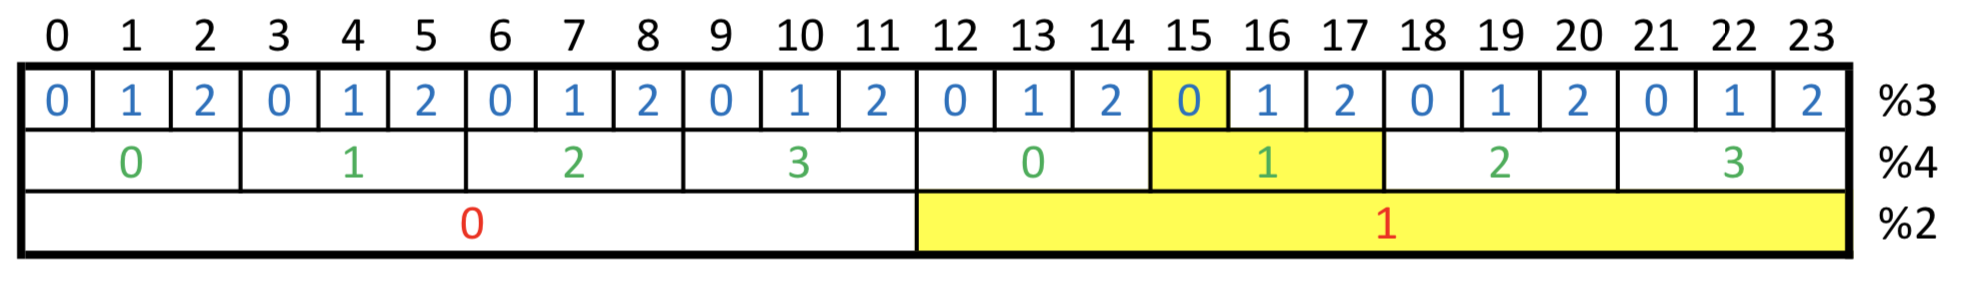
\includegraphics[origin=c,width=12cm]{../figures/interval-breakdown-final.png}}
\caption{Decomposing a Number into Constituent Ranges}
\label{fig:interval_breakdown}
\end{figure}

This technique will be applied multiple times during sequence construction to select a unique combination of values corresponding to a single integer.

\subsection{Constructing Permutations}

The construction algorithm also needs to map an individual number to a corresponding permutation of a set. Every permutation of a set can be identified by its \textit{inversion} or \textit{inversion sequence}. Loosely defined, the inversion sequence indicates how out-of-order the permutation is when compared with the original sequence. The concept of an inversion was first introduced by Hall \cite{hall_automorphisms_1962}, though we will use on Brualdi's description \cite{brualdi_introductory_2010} here.

Let $S$ be the set of numbers $\{1, 2, ..., n\}$ Suppose we have some permutation $p$ of $S$, $i_1, i_2, ..., i_n$. For each $i$, there exists some finite number of elements in $S$ whose values are greater than $i$, yet precede $i$ in $p$. This is called the inversion for $i$. An inversion sequence, $a_1, a_2, ... a_n$, is the sequence of inversions for a particular permutation of $S$.

For example, because the elements $\{1, 2, 3, 4, 5\}$ are in order, the corresponding inversion sequence for this arrangement is $\{0, 0, 0, 0, 0\}$. If we permute the sequence to obtain $\{2, 5, 4, 1, 3\}$, the associated inversion sequence is $\{3, 0, 2, 1, 0\}$. This sequence can be interpreted to mean that three elements larger than one precede one, zero elements larger than two precede two, two elements larger than three precede three, one element larger than four precedes four, and zero elements larger than five precede five. In our case, the original sequence will always be ascending; therefore, the last inversion must always be zero.

An inversion sequence can be used to generate the associated permutation by using the inversions to select where to place each element. Given an inversion sequence $a_1, a_2, ... a_n$, begin with $n$ empty locations. Beginning with $a_1$, skip $a_i$ empty locations before inserting the $i^{th}$ element of $S$. Figure \ref{fig:inversion_sequence} demonstrates this algorithm in the previous example.

\begin{figure}[b]
\centering
\centerline{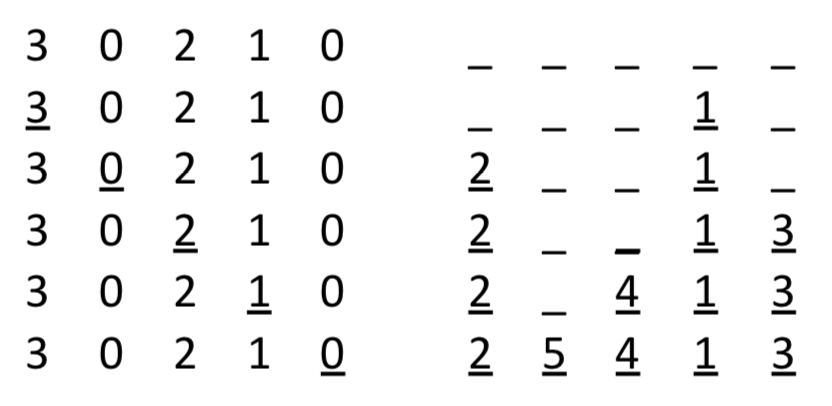
\includegraphics[origin=c,width=12cm]{../figures/inversion-sequence.png}}
\caption{Construction of a Permutation from its Inversion Sequence}
\label{fig:inversion_sequence}
\end{figure}

Finally, we can construct the inversion sequence for the $j^{th}$ permutation of a set by applying the interval mapping technique introduced in Section 5.1.1. The maximum value of each position in the inversion sequence is used to construct the intervals. To construct an inversion sequence of $n$ inversions, the set of upper bounds for the intervals is $U = \{n, n - 1, n - 2, ..., 2, 1\}$. Using interval mapping to construct an inversion sequence, we can deterministically construct any permutation of a set.

\subsection{Combinations}

We can enumerate combinations of a set of elements in a similar manner. For a combination of $r$ elements, taken from a set of $k$ elements, the multiplication principle dictates that there are $k^r$ possibilities. Applying interval mapping with $r$ intervals, each from $[0, k)$, suffices to enumerate each combination. The selected values from each interval identify the chosen items from the original set.

\section{Construction Algorithm}

Now that we have established techniques for counting solutions and constructing specific permutations and combinations based on a numeric index, we are ready to develop the full construction algorithm. The construction algorithm itself mirrors the structure of the counting formula. Each term in the counting formula becomes an upper-bound for an interval, to which interval mapping can be applied, followed by the construction of the specific permutation or combination represented by each term. At a high level, the construction process has the following steps:

\begin{enumerate}
\item Determine the total number of solutions, $s$, for the design.
\item Randomly sample an integer, $i$, from the uniform distribution in the range $[0, s)$.
\item Use interval mapping to convert $i$ into a unique combination of value selections, $R$, that identify each component of the final solution.
\item Convert each selected value in $R$ to the associated factors and levels. Record them as part of the final solution.
\item Determine the selected levels for factors in $\overline{C}_D$ by applying the corresponding predicates to the previously selected levels for basic factors.
\end{enumerate}

Accomplishing Step 1 was the subject of a previous chapter; we will not revisit that here. Step 2 relies on the \texttt{randrange} standard library function in Python 3, which produces uniformly-distributed values from an arbitrarily broad range. Step 3 is where most of the work lies, particularly in selecting the ranges for interval mapping.

\subsection{Interval Mapping for an Experimental Design}

For tier 1, 2, and 3 designs, as we saw in 4.2, there exists a partition of the factors comprised of 5 sets: $\{C_B, C_D, \overline{C}_{B_S}, \overline{C}_{B_I}, \overline{C}_D\}$. This section will describe how the selected sequence number identifies the level selections for all factors in each set. The outcome will be a set of upper bounds to which interval mapping can be applied to identify aspects of the sequence. We will use $U$ to denote the set of these upper bounds. (The lower bounds are uninteresting, as they are always $0$).

We first consider $C_B$ and $C_D$. Recall that together, these sets contain all factors that are combined with each other to form the crossing, labeled $X$ in Chapter 3. Recall also that $|X|$ governs the length of a generated trial sequence: $l = |X|$, and that there are $l!$ permutations of the sequences in $X$. Therefore, the first interval, which identifies which permutation of $X$ to use, is $l!$. Selecting a single integer from this range will identify a permutation that fully constrains the level selection for each trial for all factors in $C_B$ and $C_D$. Therefore at this point, $U = \{l!\}$.

The next set in the partition is $\overline{C}_{B_S}$, which is the set of basic factors that are \textit{not} included in the crossing but are sources of data for derived factors in the crossing. More precisely, $\overline{C}_{B_S}$ contains basic factors not in $C_B$, but that influence factors in $C_D$. Because the crossing constrains the levels selected for factors in $C_D$, it also transitively constrains potential level choices for factors in $\overline{C}_{B_S}$.

Recall from Chapter 4 that we defined $X_S$ to represent the source crossing or the set of sequences enumerating all combinations of levels for factors in $\overline{C}_{B_S}$. We also established that there is a distinct subset of $X_S$, $J_n$, that contains sequences from the source crossing that are compatible with the $n^{th}$ sequence in $X$. We also defined $S$ to be the set of these subsets. A distinct interval for each of these subsets is required. Therefore we add $l$ values to $U$: one for the size of each subset in $S$. $U$ will now contain $l + 1$ elements: $U = \{l!, |J_1|, |J_2|, ..., |J_l|\}$.

Lastly,\footnote{$\overline{C}_D$ has been skipped, but values for factors in this set are governed by other basic factors and will be determined in step 5. No additional intervals need be computed to account for factors in this set.} we consider $\overline{C}_{B_I}$. Recall that $\overline{C}_{B_I}$ represents the set of basic factors that are completely independent, meaning they are not governed by any factors in $C_D$. Because they are completely independent, every possible $l$-combination of levels for each factor in $\overline{C}_{B_I}$ is valid. Therefore an interval is added for each factor $f$ with upper bound $|f|^l$. (Recall that $|f|$ denotes the number of levels of factor $f$.) $U$ is now complete:

\[
U = \{ l!, |J_1|, |J_2|, ..., |J_l|, |f_1|^l, |f_2|^l, ..., |f_i|^l\}
\]

Where $f_i$ represents the $i^{th}$ factor in $\overline{C}_{B_I}$. Unsurprisingly, the upper bounds in $U$ are the same values which were multiplied together in Chapter 4 to produce the total solution count.

Once a sequence number $i$ has been selected (Step 2), and $U$ has been constructed, interval mapping is applied to map $i$ into its constituent pieces representing the final sequence. The mapped value from each range identifies a specific permutation or combination for that aspect of the sequence. The bulk of the trial sequence can be assembled using these values and methods for constructing indexed permutations and combinations. Finally, we select levels for factors in $\overline{C}_D$ by applying their corresponding predicates to the selected levels for each trial.


\subsection{Mapping Selected Values to Sequences}

Once interval mapping has produced values for each interval, SweetPea must convert the value into its associated permutation or combination in the original design. The first value, $U_0$, identifies a particular permutation of the crossing, the next $l$ values, $U_1$ to $U_l$, identify a particular source combination for the $l^{th}$ trial in the sequence,\footnote{Ordering is important here due to the association between valid source combinations and specific sequences in the crossing. The same permutation that scrambles the crossing must also be applied to the set of source combinations to preserve the integrity of the association.} and the remaining values beginning with $U_{l+1}$ identify particular $l$-combinations to be used for each independent basic factor in the sequence. Each of these three types of values identifies a permutation or combination that spans a different dimension of the final sequence. Figure \ref{fig:sequence_dimensions} gives a visual representation to assist the reader.

\begin{figure}[t]
\centering
\centerline{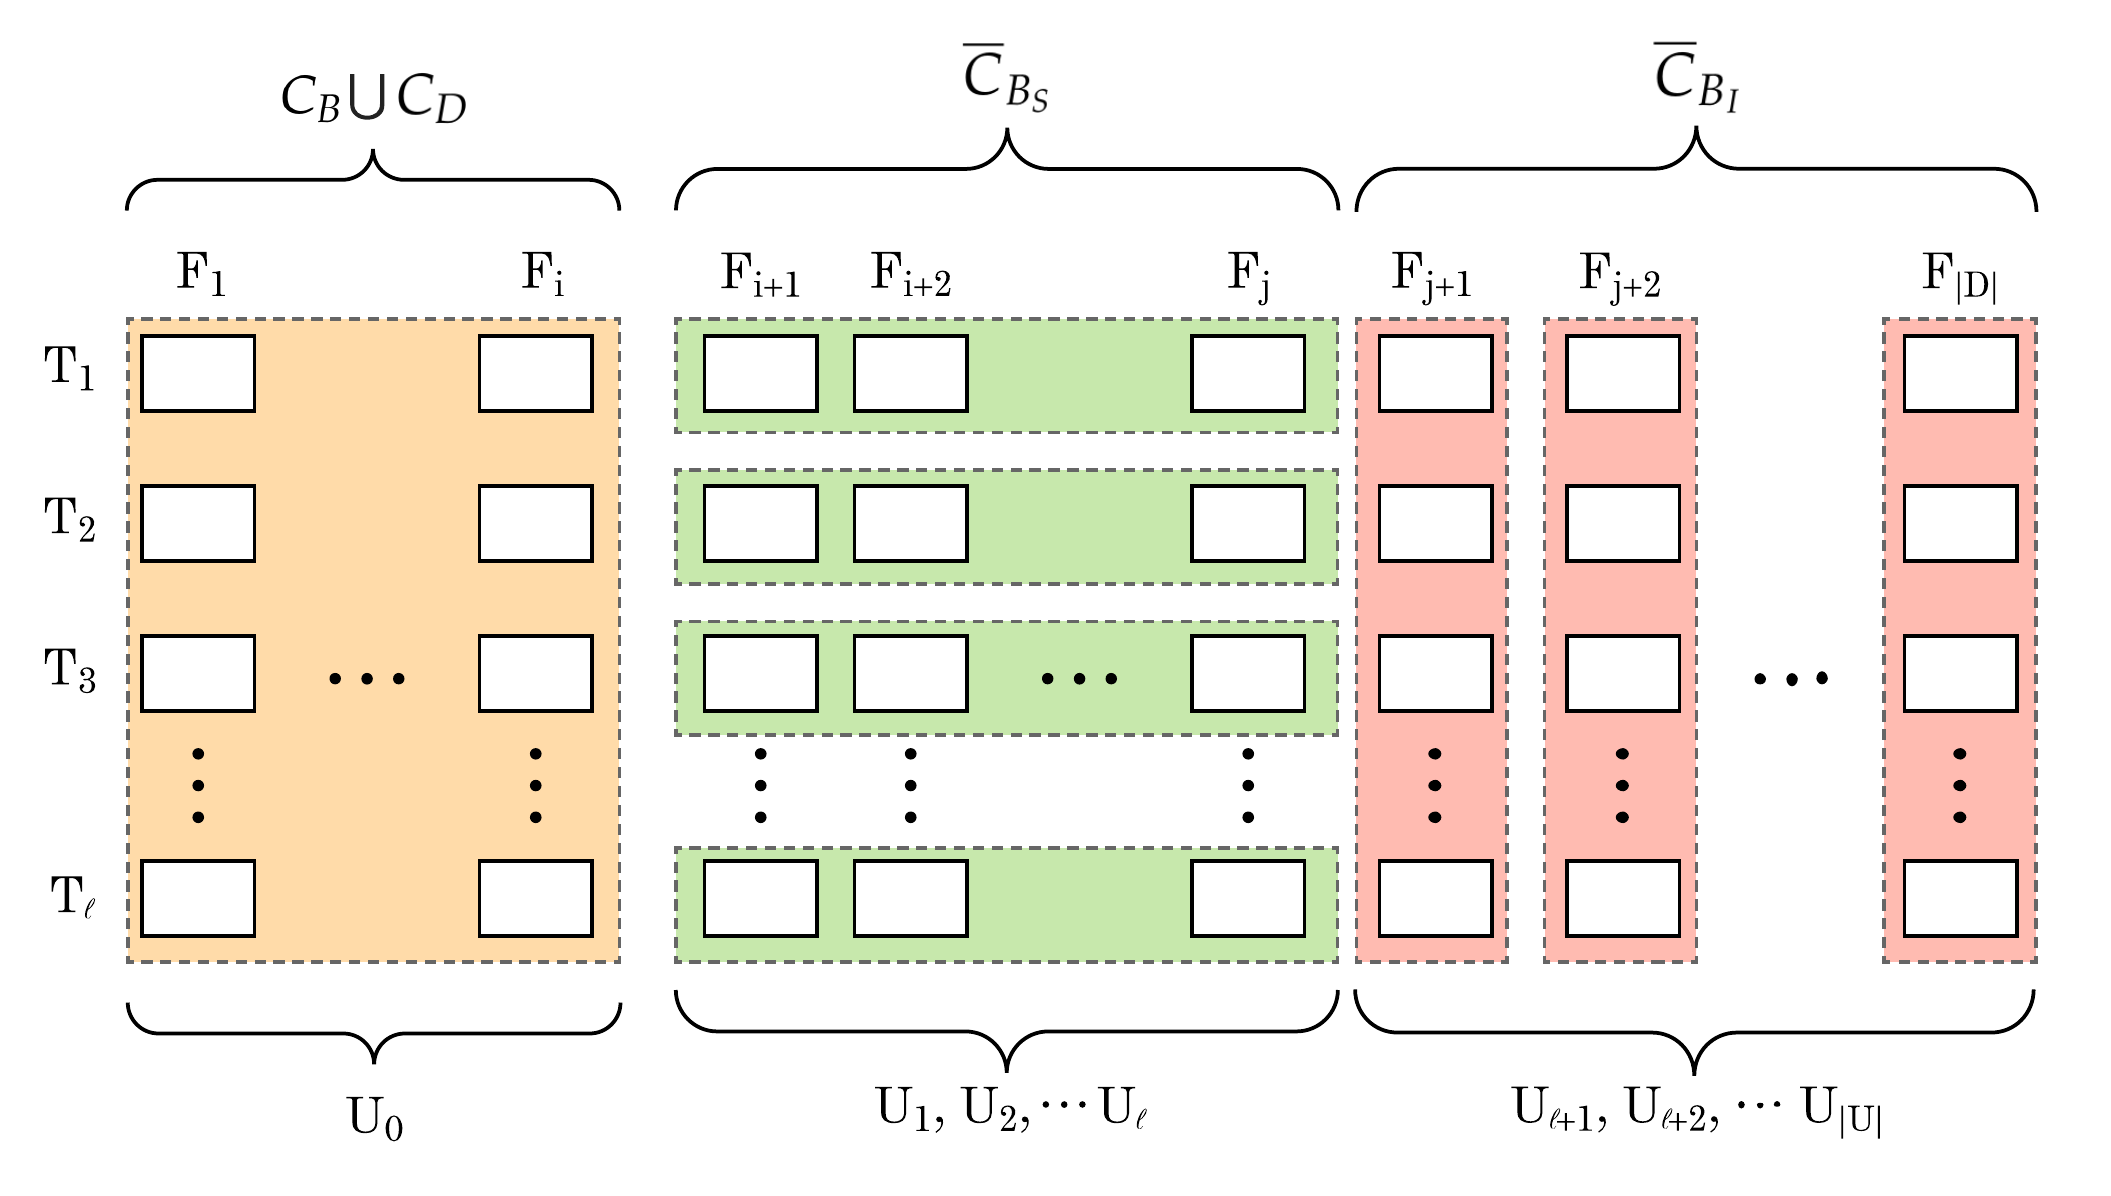
\includegraphics[origin=c,width=12cm]{../figures/sequence-dimensions.png}}
\caption{Dimensionality of Interval Values}
\label{fig:sequence_dimensions}
\end{figure}

The selected permutation value ($U_0$) is converted to a unique inversion sequence by again applying interval mapping. The inversion sequence is then used to construct the associated permutation using the technique introduced in Section 5.1.2. The algorithm then produces level values by using each integer in the permutation as an index into the sequences in $X$.

The algorithm converts the selected values for independent basic factors ($U_{l+1}$ to $U_{|U|}$) similarly. Each selected value identifies a combination index, which the algorithm converts to a set of values using interval mapping. Each value is an index into the list of levels for the associated factor. % TODO - does this need more?

Lastly, the algorithm must convert the selected values for source combinations ($U_1$ to $U_l$). These are more complex than the previous conversions because a set of valid source combinations is associated with an individual trial in the sequence. It would be incorrect to select a source combination from the $n^{th}$ set of valid source combinations for the $n^{th}$ trial, because the permutation may have shifted the position of the original $n^{th}$ trial in the sequence. Therefore care must be taken to preserve this association. The algorithm preserves this association by using the original trial index when selecting the set of valid source combinations. Figure \ref{fig:source_combinations} outlines the entire mapping process.


\begin{figure}[t]
\centering
\centerline{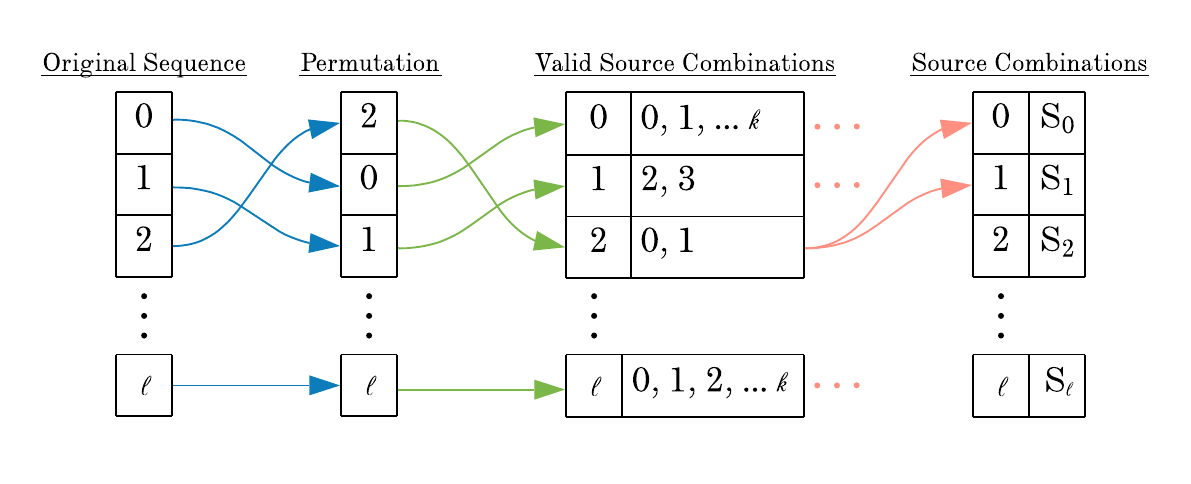
\includegraphics[origin=c,width=12cm]{../figures/source-combination-mapping.png}}
\caption{Selecting Valid Source Combinations}
\label{fig:source_combinations}
\end{figure}

For example, if the selected permutation places the original crossing value for trial number 2 in the zeroth position in the sequence (trial 0), then the source combination for trial 0 must also be selected from the valid source combinations originally generated for trial number 2.


\section{Example}

We will now use this method to construct a single solution to the design from the counting example in the previous chapter. We will choose a solution at random from $[1, 5760]$: $2590$.

First, we compute the set of value selections, $R$, for the $2,590^{th}$ solution. In order to do this, we first compute $U$, the set of upper-bounds for each range. The first upper bound is the number of permutations, $l!$, for the design. For this example, this was determined to be $720$. Next, we add the size of each subset of $S$ (See Table \ref{tab:example_s}) to $U$ to select valid source combinations. $U$ now contains 7 elements: $U = \{720, 1, 2, 1, 2, 1, 2\}$. Because $\overline{C}_{B_I} = \emptyset$ and $\overline{C}_D = \emptyset$ in this example, there are no other bounds to compute, so $U$ is complete.

When interval mapping is applied to $2590$ to generate values from these ranges, $R$ is determined to be $R = \{430, 0, 1, 0, 1, 0, 0\}$. With $R$ computed, we can now use the selected values to generate the correct permutation, and then select level combinations for the remaining factors.

To generate the $430^{th}$ permutation, we first construct the $430^{th}$ inversion sequence by again applying interval mapping with $U = \{6, 5, 4, 3, 2, 1\}$. This yields $\{4, 1, 2, 0, 1, 0\}$ as the $430^{th}$ inversion sequence. Applying the algorithm to convert this sequence to its corresponding permutation, we obtain $\{3, 1, 5, 2, 0, 4\}$. The crossing, $X$, was identified in Chapter 4 to be:

\begin{align*}
X = \{(red, yes), (red, no), (green, yes), (green, no), (blue, yes), (blue, no)\}
\end{align*}

The permutation $\{3, 1, 5, 2, 0, 4\}$ therefore corresponds to:

\[
    \{(green, no), (red, no), (blue, no), (green, yes), (red, yes), (blue, yes)\}
\]


We have now selected levels for factors in $C_B$ and $C_D$. The only remaining factor is \texttt{text}, which is in $\overline{C}_{B_S}$. The source combination selections from $R$ for this factor were $\{0, 1, 0, 1, 0, 0\}$. We then use the values from the permutation as indices to select both the source combination list and the selected value from that list for each trial. This process is represented visually in Figure \ref{fig:source_combinations}. In Chapter 4 we established the set of source combination lists to be:

\[
S = \{(red), (green, blue), (green), (red, blue), (blue), (red, green)\}
\]

The first value of the permutation is $3$, which corresponds to the source combination list $(red, blue)$, and a value selection of $1$. Therefore the level selected for \texttt{text} in the first trial is $blue$. Following the same pattern, the level selections for \texttt{text} in each trial are:

\[
  \{blue, blue, red, green, red, blue\}
\]

Another perspective is that we are applying the same permutation computed previously to the list of level selections and the list of source combinations, before doing the final lookup. Combining all level selections yields a complete trial sequence which is shown in Table \ref{tab:example_trial_sequence}.

\begin{table}[b]
  \centering
  \caption{The $2590^{th}$ Trial Sequence}
\begin{tabular}{rccc}
\multicolumn{1}{c}{Trial} & Color   & Text    & Congruent \\ \hline
1                         & $green$ & $blue$  & $no$      \\
2                         & $red$   & $blue$  & $no$      \\
3                         & $blue$  & $red$   & $no$      \\
4                         & $green$ & $green$ & $yes$     \\
5                         & $red$   & $red$   & $yes$     \\
6                         & $blue$  & $blue$  & $yes$
\end{tabular}
\label{tab:example_trial_sequence}
\end{table}


% \begin{align*}
% i = 2,590 &&  R_1 = 2,590 \bmod 720 = 430 && i = \Bigl\lfloor \frac{2,590}{720} \Bigr\rfloor = 3 \\
% i = 3     &&  R_2 = 3 \bmod 1 = 0         && i = \Bigl\lfloor \frac{3}{1} \Bigr\rfloor = 3 \\
% i = 3     &&  R_3 = 3 \bmod 1 = 0         && i = \Bigl\lfloor \frac{3}{1} \Bigr\rfloor = 3 \\
% i = 3     &&  R_4 = 3 \bmod 1 = 0         && i = \Bigl\lfloor \frac{3}{1} \Bigr\rfloor = 3 \\
% i = 3     &&  R_5 = 3 \bmod 2 = 1         && i = \Bigl\lfloor \frac{3}{2} \Bigr\rfloor = 1 \\
% i = 1     &&  R_6 = 1 \bmod 2 = 1         && i = \Bigl\lfloor \frac{1}{2} \Bigr\rfloor = 0 \\
% i = 0     &&  R_7 = 0 \bmod 2 = 0         &&                                               \\
% \end{align*}

% To generate the $430^{th}$ permutation, we first construct the $430^{th}$ inversion sequence by applying interval mapping with $U = \{6, 5, 4, 3, 2, 1\}$:

% \begin{align*}
% i = 430  &&  R_1 = 430 \bmod 6 = 4  &&  i = \Bigl\lfloor \frac{430}{6} \Bigr\rfloor = 71 \\
% i = 71   &&  R_2 = 71 \bmod 5 = 1   &&  i = \Bigl\lfloor \frac{71}{5} \Bigr\rfloor = 14  \\
% i = 14   &&  R_3 = 14 \bmod 4 = 2   &&  i = \Bigl\lfloor \frac{14}{4} \Bigr\rfloor = 3   \\
% i = 3    &&  R_4 = 3 \bmod 3 = 0    &&  i = \Bigl\lfloor \frac{3}{3} \Bigr\rfloor = 1    \\
% i = 1    &&  R_5 = 1 \bmod 2 = 1    &&  i = \Bigl\lfloor \frac{1}{2} \Bigr\rfloor = 0    \\
% i = 0    &&  R_6 = 0 \bmod 1 = 0    &&                                                   \\
% \end{align*}




\section{Handling Constraints}

Recall that the complexity gradation did not account for the external constraints that may be part of the design. Such constraints typically enforce some rule regarding repetition of particular characteristics. For example, in the design for Stroop experiments, it is common to apply a constraint that requires that the generated sequence never contain two consecutive congruent trials. Constraints may be applied to the levels of derived factors as well; therefore, the user may impose practically any condition upon the generated sequence.

In the future, the counting and construction algorithms could be enhanced to account for these constraints. Such improvements will be discussed further in Chapter 6. In the meantime, however, rejection sampling is applied to ensure that the algorithm does not ever return sequences that violate constraints. The generated sample is checked against all repetition constraints in the design to verify that no violations exist. As will be seen in the next section, this performs adequately in practice.


\section{Benchmarks}

Of the ten benchmarks designs that were introduced in Chapter 3, four can be classified as tier 1, 2, or 3 designs: \texttt{stroop-2}, \texttt{stroop-3}, \texttt{stroop-4}, \texttt{stroop-5}. We will repeat the benchmarks for those designs here using this construction approach to sampling. We will also introduce a few additional designs involving variations on the Stroop design to demonstrate the scalability of this approach and the empirical performance of the rejection sampling phase. Table \ref{tab:benchmark_experiments_construction} reviews the basic experiment data for each benchmark design. Table \ref{tab:sampling_metrics} summarizes the time required to generate 10,000 samples for each design using a single core, as well as the average number of rejections per sample. (Rejections caused by constructing a trial sequence that violated external constraints.)

% Extra constraints:
% constraints = [AtMostKInARow(1, ("congruent?", "yes")), AtMostKInARow(3, color), AtMostKInARow(3, text)]

\begin{table}[b]
  \centering
  \caption{Benchmark Experiments for Sequence Construction}
\begin{tabular}{|c|c|c|c|c|}
\hline
\multicolumn{1}{|l|}{Experiment Name} & Length          & Unconstrained Solutions  & Single Sample  \\ \hline
stroop-2                              & 4               & 24                       & 0.0009s        \\ \hline
stroop-3                              & 9               & 362,880                  & 0.003s         \\ \hline
stroop-4                              & 16              & 20,922,789,888,000       & 0.007s         \\ \hline
stroop-5                              & 25              & $\approx 2^{83}$         & 0.016s         \\ \hline
stroop-10                             & 100             & $\approx 2^{524}$        & 0.170s         \\ \hline
stroop-20                             & 400             & $\approx 2^{2886}$       & 2.729s         \\ \hline
stroop-20-extra-constraints           & 400             & $\approx 2^{2886}$       & 3.234s         \\ \hline
\end{tabular}
\label{tab:benchmark_experiments_construction}
\end{table}

Even for huge designs, this approach constructs a single random sample exceptionally quickly.

\begin{table}[t]
  \centering
  \caption{Sampling Metrics}
\begin{tabular}{|c|c|c|c|c|}
\hline
\multicolumn{1}{|l|}{Experiment Name} & 10,000 Samples & Avg. Rejections/Sample  \\ \hline
stroop-2                              & 8.763s         & 0.982                   \\ \hline
stroop-3                              & 29.323s        & 1.393                   \\ \hline
stroop-4                              & 72.882s        & 1.53
8                   \\ \hline
stroop-5                              & 155.699s       & 1.589                   \\ \hline
stroop-10                             & 1908.598s      & 1.698                   \\ \hline
stroop-20                             & 26064.417s     & 1.684                   \\ \hline
stroop-20-extra-constraints           & 27338.002s     & 1.898                   \\ \hline
\end{tabular}
\label{tab:sampling_metrics}
\end{table}

Generating a large number of samples can still take a significant amount of time. However, because samples can be generated independently of one another, this algorithm can be easily parallelized for a linear speedup in the number of available cores.
